\documentclass{beamer}

% --- Pacchetti per i font personalizzati ---
\usepackage{fontspec} % Richiede XeLaTeX o LuaLaTeX
\setsansfont{Raleway} % Font principale
\setmainfont{Raleway}
\newfontfamily\titlefont{Rokkitt} % Font per i titoli

% --- Definizione del tema ---
\usetheme{default} % Tema di base
\usecolortheme{seagull} % Colori semplici

% --- Configurazione dei colori personalizzati ---
\definecolor{linuxGreen}{RGB}{57,181,74} % Verde open source
\definecolor{linuxGray}{RGB}{85,87,83} % Grigio scuro

% --- Logo Tux in alto a sinistra ---
\setbeamertemplate{logo}{%
	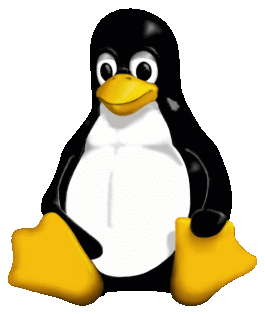
\includegraphics[height=0.8cm]{images/Tux.png} % Immagine di Tux; sostituire con il percorso effettivo
}

% --- Struttura e colore delle slide ---
\setbeamercolor{frametitle}{bg=linuxGreen, fg=white}
\setbeamercolor{title}{fg=linuxGreen}
\setbeamercolor{structure}{fg=linuxGray}
\setbeamercolor{section in head/foot}{bg=linuxGreen, fg=white}
\setbeamercolor{author in head/foot}{bg=linuxGray, fg=white}

% --- Personalizzazione dei titoli con font Rokkitt ---
\setbeamerfont{title}{family=\titlefont, size=\Huge}
\setbeamerfont{frametitle}{family=\titlefont, size=\LARGE}
\setbeamerfont{section title}{family=\titlefont}

% --- Personalizzazione del titolo della slide ---
\setbeamertemplate{frametitle}{%
	\begin{beamercolorbox}[wd=\paperwidth,ht=2.5ex,dp=1ex,leftskip=0.3cm]{frametitle}
		\usebeamerfont{frametitle}\insertframetitle
	\end{beamercolorbox}
}

% --- Footer con data e titolo sezione ---
\setbeamertemplate{footline}{%
	\begin{beamercolorbox}[wd=\paperwidth,ht=2.5ex,dp=1ex,leftskip=0.3cm,rightskip=0.3cm]{section in head/foot}
		Linux Day 26 Ottobre 2024 \hfill \insertshorttitle \hfill \insertframenumber/\inserttotalframenumber
	\end{beamercolorbox}
}

% --- Struttura della presentazione ---
\title{Introduzione al Mondo Open Source}
\author{Relatore: Davide Isoardi}
\date{Linux Day 26 Ottobre 2024}
\newcommand{\license}{Creative Commons Attribution-ShareAlike 4.0 International (CC BY-SA 4.0)}

% --- Inizio del documento ---
\begin{document}
	
	% Slide di apertura
	\begin{frame}
		\titlepage
	\end{frame}
	
	% Slide dell'indice dei contenuti
	\begin{frame}{Indice dei Contenuti}
		\tableofcontents
	\end{frame}
	
	% --- Sezione Premesse ---
	\section{Premesse}
	
	\begin{frame}{Stack ISO/OSI}
		\begin{itemize}
			\item Modello di riferimento per la comunicazione in rete.
			\item Suddiviso in 7 livelli, ognuno con funzioni specifiche.
			\item Garantisce interoperabilità tra sistemi di produttori diversi.
		\end{itemize}
	\end{frame}
	
	\begin{frame}{Overview su Home Assistant}
		\begin{itemize}
			\item Piattaforma open-source per l'automazione domestica.
			\item Supporta numerosi protocolli e dispositivi IoT.
			\item Sviluppata per integrare vari sistemi in una piattaforma unica.
		\end{itemize}
	\end{frame}
	
	% --- Sezione IoT e Onde Radio ---
	\section{IoT e Onde Radio}
	
	\begin{frame}{Z-wave}
		\begin{itemize}
			\item Progettato specificamente per la domotica.
			\item Basso consumo energetico e frequenza sub-GHz.
			\item Supporta reti mesh per aumentare il raggio di copertura.
		\end{itemize}
	\end{frame}
	\begin{frame}{Z-Wave (dettagli tecnici)}
		\begin{itemize}
			\item Frequenza di operazione: 868 MHz (Europa), 908 MHz (Stati Uniti)
			\item Canali configurabili: 1-232
			\item Range: fino a 100 m indoor, fino a 3 km outdoor
			\item Data rate: up to 40 kbps
			\item Power consumption: low power devices (LPD) <1mW, full-function devices (FFD) <12mW
			\item Encryption: S2 and AES-128
			\item Dimensioni oggetto interferente:
				La lunghezza d'onda di 3,5 cm (868 MHz) e 3,3 cm (908 MHz) è importante per capire le dimensioni minime degli oggetti che possono interferire con il segnale radio.
		\end{itemize}
	\end{frame}
	
	\begin{frame}{ZigBee}
		\begin{itemize}
			\item Protocollo wireless a bassa potenza, ideale per dispositivi a batteria.
			\item Ampiamente usato in domotica e automazione.
			\item Frequenza 2.4 GHz, con supporto per reti mesh.
		\end{itemize}
	\end{frame}
	\begin{frame}{ZigBee (dettagli tecnici)}
		\begin{itemize}
			\item Frequenza di operazione: 2,4 GHz
			\item Canali configurabili: 16 (USA), 10 (Europe)
			\item Range: fino a 100 m indoor, fino a 3 km outdoor
			\item Data rate: up to 250 kbps
			\item Power consumption: low power devices (LPD) <1mW, full-function devices (FFD) <15mW
			\item Encryption: AES-128, DES
			\item Dimensioni oggetto interferente:
				La lunghezza d'onda di 12,5 cm è importante per capire le dimensioni minime degli oggetti che possono interferire con il segnale radio.
		\end{itemize}
	\end{frame}
	
	\begin{frame}{BLE (Bluetooth Low Energy)}
		\begin{itemize}
			\item Versione ottimizzata di Bluetooth per basso consumo.
			\item Utilizzato in dispositivi come sensori e wearable.
			\item Raggio corto, ma facilmente integrabile grazie alla sua diffusione.
		\end{itemize}
	\end{frame}
	\begin{frame}{Bluetooth Low Energy (BLE) (dettagli tecnici)}
		\begin{itemize}
			\item Frequenza di operazione: 2,4 GHz
			\item Canali configurabili: 40 (3 MHz di spaziatura)
			\item Range: fino a 100 m indoor, fino a 1 km outdoor
			\item Data rate: up to 2 Mbps
			\item Power consumption: low power devices (LPD) <10mW, full-function devices (FFD) <30mW
			\item Encryption: AES-128
			\item Dimensioni oggetto interferente: la lunghezza d'onda di 12 cm è importante per capire le dimensioni minime degli oggetti che possono interferire con il segnale radio.
		\end{itemize}
	\end{frame}
	
	\begin{frame}{CoAP (Constrained Application Protocol)}
		\begin{itemize}
			\item Protocollo di comunicazione per IoT su reti a bassa larghezza di banda.
			\item Supporta trasmissione dati RESTful simile a HTTP.
			\item Ideale per dispositivi con risorse limitate.
		\end{itemize}
	\end{frame}
	
	\begin{frame}{WiFi}
		\begin{itemize}
			\item Protocollo di rete wireless diffuso e ad alta velocità.
			\item Ampia larghezza di banda e bassa latenza.
			\item Ideale per dispositivi che necessitano di velocità, ma a scapito del consumo energetico.
		\end{itemize}
	\end{frame}
	\begin{frame}{WiFi (dettagli tecnici)}
		\begin{itemize}
			\item Frequenza di operazione: 2,4 GHz e 5 GHz
			\item Canali configurabili: varia in base al paese e alla regione
			\item Range: fino a 100 m indoor, fino a 1 km outdoor
			\item Data rate: up to 600 Mbps (802.11ac) and up to 9.6 Gbps (802.11ad)
			\item Power consumption: varia in base al tipo di dispositivi e alla loro potenza di trasmissione
			\item Encryption: WPA2, WPA3, AES-128, AES-256
			\item Dimensioni oggetto interferente: la lunghezza d'onda di 12 cm è importante per capire le dimensioni minime degli oggetti che possono interferire con il segnale radio.
		\end{itemize}
	\end{frame}
	
	\begin{frame}{LoRaWAN}
		\begin{itemize}
			\item Protocollo di rete per dispositivi IoT a lungo raggio.
			\item Utilizza modulazione LoRa (Long Range) per comunicazioni a basso consumo e lunga distanza.
			\item Ideale per applicazioni IoT in ambienti distribuiti e smart cities.
			\item Supporta reti pubbliche e private con una topologia a stella.
		\end{itemize}
	\end{frame}
	\begin{frame}{LoRaWAN (dettagli tecnici)}
		\begin{itemize}
			\item Frequenza di operazione: 868 MHz, 923 MHz
			\item Canali configurabili: varia in base al paese e alla regione
			\item Range: fino a 15 km outdoor, fino a 5 km indoor
			\item Data rate: up to 50 kbps
			\item Power consumption: low power devices (LPD) <30mW, full-function devices (FFD) <100mW
			\item Encryption: AES-128, OTAA, ABP
			\item Dimensioni oggetto interferente: la lunghezza d'onda di 12 cm è importante per capire le dimensioni minime degli oggetti che possono interferire con il segnale radio.
		\end{itemize}
	\end{frame}
	
	\section{Protocolli di interoperabilità}
	\begin{frame}{Protocolli di Interoperabilità: Matter e Thread}
		\begin{itemize}
			\item Matter e Thread operano a un livello superiore rispetto ai protocolli radio (ad esempio WiFi, Zigbee) nella piramide OSI:
			\begin{itemize}
				\item Protocolli radio (WiFi, Zigbee): Layer 2 (Data Link)
				\item Matter e Thread: Layer 3 (Network)
			\end{itemize}
			\item Sono focalizzati sulla comunicazione device-to-device, piuttosto che su comunicazione device-to-cloud o cloud-to-cloud
			\item Consentono l'integrazione smagliante di dispositivi da diverse aziende e con diverse capacità
		\end{itemize}
	\end{frame}
	
	\begin{frame}{Matter}
		\begin{itemize}
			\item Protocollo unificato per l'interoperabilità dei dispositivi IoT.
			\item Supporta vari protocolli come WiFi, Ethernet e Thread.
			\item Sviluppato dal gruppo CSA (Connectivity Standards Alliance).
		\end{itemize}
	\end{frame}
\begin{frame}{Matter - Dettagli Tecnici 1}
	\begin{itemize}
		\item Comunicazione device-to-device:
		\begin{itemize}
			\item Utilizza protocollo UDP esteso (Matter UDP)
			\item Utilizza indirizzo IP come destinazione
			\item Non richiede creazione di connessioni TCP per inviare dati
		\end{itemize}
		\item Source Route:
		\begin{itemize}
			\item Ogni dispositivo mantiene routing table con indirizzi IP dei dispositivi vicini e capacità di routing
		\end{itemize}
	\end{itemize}
\end{frame}
\begin{frame}{Matter - Dettagli Tecnici 2}
	\begin{itemize}
		\item Multicast:
		\begin{itemize}
			\item Pacchetti UDP possono essere inviati a più dispositivi contemporaneamente utilizzando multicast
			\item Riduce stato delle reti e migliora velocità di trasmissione
		\end{itemize}
		\item Neighbor Discovery:
		\begin{itemize}
			\item Ogni dispositivo scopre dispositivi vicini attraverso processo chiamato "neighbor discovery"
			\item Utilizza pacchetti UDP specifici per scambiare informazioni sulla presenza e sulle capacità dei dispositivi
		\end{itemize}
		\item Frame Format:
		\begin{itemize}
			\item Pacchetti UDP hanno struttura speciale con campo di destinazione (indirizzo IP del dispositivo destinatario) e campo di contenuto (dati da trasmettere)
		\end{itemize}
	\end{itemize}
\end{frame}

	\begin{frame}{Thread}
		\begin{itemize}
			\item Protocollo di rete wireless basato su IPv6.
			\item Progettato per la comunicazione sicura tra dispositivi IoT.
			\item Supporta reti mesh, migliorando l'affidabilità e riducendo i consumi.
		\end{itemize}
	\end{frame}
	
% --- Threads (Dettagli Tecnici) ---
\begin{frame}
	\frametitle{Thread: Dettagli Tecnici}
	\begin{itemize}
		\item Funziona principalmente al livello network (livello 3 ISO/OSI) su IPv6.
		\item Ottimizzato per dispositivi a basso consumo, ideale per sensori e attuatori alimentati a batteria.
		\item Ha un range di azione: 30-100 metri tra i nodi, con possibilità di estensione grazie alla topologia mesh.
		\item Architettura di rete:
		\begin{itemize}
			\item Router: Gestiscono il traffico tra i dispositivi.
			\item End Device: Dispositivi che non partecipano al routing, ma utilizzano la rete (es. sensori).
			\item Leader: Un dispositivo che gestisce l'allocazione degli indirizzi nella rete.
			\item Border Router: Connette la rete Thread ad altre reti IP (come Wi-Fi o Ethernet).
		\end{itemize}
		\item Utilizza la crittografia AES-128 per garantire la sicurezza delle comunicazioni.
		\item Supporta fino a 250 dispositivi su una singola rete.
	\end{itemize}
\end{frame}

% --- Threads e Matter ---
\section{Thread e Matter}
\begin{frame}
	\frametitle{Thread e Matter}
	\begin{itemize}
		\item Thread è indipendente: Può operare come protocollo di rete autonomo.
		\item Matter utilizza Thread: Matter sfrutta Thread come infrastruttura di rete mesh, ma non è limitato a esso.
		\item Thread per Matter: Matter utilizza Thread per i dispositivi a basso consumo energetico in una rete locale.
		\item Altri protocolli supportati da Matter: Oltre a Thread, Matter funziona anche su Wi-Fi e Ethernet.
		\item Interoperabilità: Matter facilita l'interoperabilità tra dispositivi basati su Thread e quelli su altre reti, grazie al supporto IP di Thread.
	\end{itemize}
\end{frame}
	% --- Sezione Deadmatch ---
	\section{Deadmatch}
	
	\begin{frame}{Confronto tra i protocolli visti}
		\begin{itemize}
			\item Z-Wave e ZigBee: ideali per reti mesh a basso consumo.
			\item WiFi: maggiore velocità, ma più consumo energetico.
			\item BLE: ottimo per corto raggio e basso consumo.
			\item Matter e Thread: offrono interoperabilità e connessione sicura tra dispositivi.
		\end{itemize}
	\end{frame}
	
	\begin{frame}{Quando usare e quando evitare i protocolli}
		\begin{itemize}
			\item Z-Wave e ZigBee: perfetti per sensori e automazione domestica.
			\item WiFi: adatto per dispositivi fissi con alimentazione continua.
			\item BLE: ideale per dispositivi portatili con batteria.
			\item Matter e Thread: ottimi per integrazioni future-proof e sicurezza.
		\end{itemize}
	\end{frame}
	
	% --- Slide finale con licenza e ringraziamenti ---
	\section*{Licenza e Ringraziamenti}
	\begin{frame}{Licenza e Ringraziamenti}
		\begin{center}
			\textbf{Licenza:} \license % Testo della licenza centrato
			
			\vspace{1em}
			
			Questa presentazione è rilasciata sotto la licenza \license. Sentiti libero di condividere e adattare il contenuto rispettando i termini della licenza.
			
			\vspace{1.5em}
			
			
\includegraphics[width=0.2\textwidth]{images/cc-by-sa.png} % Logo Creative Commons, ridotto e centrato
			
			\vspace{1.5em}
			
			\textbf{Ringraziamenti:} Un ringraziamento speciale all'Italian Linux Society per il supporto alla community open source.
		\end{center}
	\end{frame}
	
\end{document}
